\begin{quote}
\emph{Promise is given that the purely mechanical difficulties connected with the
handling of great quantities of data can be overcome so that the computational
time factor will eventually cease to be the unsurmountable obstacle to the
practical realizations of a program of numerical forecasting.} --Jule Charney
\end{quote}

Ocean currents have influenced humanity since the beginning of time, both
through the effects ocean currents have on climate, but also through the effects
they have on human travel. Vikings and Polynesians both made use of ocean
currents in their exploration \cite{Dijkstra08, Ingstad}. The Vikings used the
ocean currents to travel between Europe and the Americas \cite{Ingstad}. In
fact, the Vikings were able to sail all along the Greenland coast, because of a
lack of ice bergs caused by a more northerly reaching Gulf Stream, which receded
a century later \cite{Morner95}.

The first documentation of ocean currents were made by Christopher Columbus
(1492-1494), Vasco da Gama (1497-1499), and Ferdinand Magellan (1519-1522)
\cite{Dijkstra08, Vallis06}. In fact, the Gulf Stream was first mapped by
Benjamin Franklin in 1769 (\autoref{fig:Franklin}) \cite{Dijkstra08, Vallis06}.
The first instrumental observations of ocean currents on a global scale were
begun by the HMS \emph{Challenger} in 1872 when she set sail for over three
years around the world \cite{Siedler01}.

\begin{figure}%[H]
  \begin{center}
    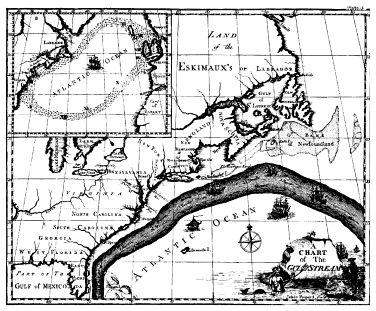
\includegraphics[scale=0.5]{Figures/Franklin-Folger.png}
    \caption{Map of the Gulf Stream by Franklin-Folger, 1769. Image courtesy of
      NOAA.gov.}
    \label{fig:Franklin}
  \end{center}
\end{figure}

In more recent times we read of plans for shipping through the Northwestern
Passage, which until recently had been closed by sea ice. Numerical climate
models predicted that the passage would eventually open, however the passage has
opened much earlier than anticipated \cite{NatGeo}.

The climate system is driven by energy from the sun. This solar energy is
transferred from the low latitudes to the high latitudes via radiative processes,
and oceanic and atmospheric circulations. The oceans have two important roles in
the climate system: \begin{inparaenum}[1)]\item They store and release heat
seasonally, and \item they transport heat around the globe by their large scale
currents \cite{Winton2003}. \end{inparaenum}  The oceans make up approximately
$71\%$ of the Earth's surface, therefore the absorption of solar energy is
dominated by the oceans.  Thus, climate variability is, to a large extent, an
ocean-related phenomenon \cite{Siedler01}. In fact, the oceans transport 3.2
petawatts from the tropics \cite{Trenberth2001}. According to Winton
\cite{Winton2003} the lack of this northward transport of heat would result in
a planet blanketed by a sea of ice.

Additionally, we see that ocean circulation changes are strongly linked to
changes in climate \cite{Morner95, Siedler01}. In fact, the cold periods in
Western Europe during the time periods 1440-1460, 1687-1703, and 1808-1821 can
all be linked to a southward deflection of the Gulf Stream and a southward
penetration of Arctic cold water \cite{Morner95}.

The large scale ocean flows are characterized by three major features: the wind
forcing, the stratification, and the effects of rotation \cite{Majda, Vallis06}.
Annual mean wind patterns, where winds are westward near the equator and
eastward at the midlatitudes \cite{Dijkstra08}, drive the subtropical and
subpolar gyres, which correspond to the strong, persistent, sub-tropical and
sub-polar western boundary currents: in the North Atlantic (the Gulf Stream and
the Labrador Current), in the South Atlantic (the Brazil and the Falkland
Currents), in the North Pacific (the Kuroshio and the Oyashio Currents), in the
South Pacific (East Australia Current) and in the Indian Ocean (the Agulhas
Current) \cite{Dijkstra08,Vallis06}. These major ocean currents are depicted in
\autoref{fig:Currents} \cite{Haidvogel1999}. One of the common features of these
gyres is that they display strong western boundary currents, weaker interior
flows, and weak eastern boundary currents. It is these wind-driven ocean
circulations that play a significant role in climate dynamics
\cite{Beesley2008,Dijkstra05,Ekman1905,Ghil08}.

\begin{figure}%[H]
  \begin{center}
    \includegraphics[scale=0.65]{Figures/WindDrivenCurrentsNOAA.pdf}%Currents.pdf}
    \caption{The large scale surface currents of the ocean. Image courtesy of
      NOAA.gov.}
    \label{fig:Currents}
  \end{center}
\end{figure}

